

\section{Background}
\label{sec:background}


This section provides the background knowledge, including machine unlearning methods and AI fairness metrics.

\subsection{Machine Unlearning Methods}
\label{sec:unlearning}


The classification problem is a type of task that many machine learning systems aim to solve and in which machine unlearning can be leveraged.
Given a dataset of input-output pairs $\mathcal{D}= (x, y) \in \mathcal{X} \times \mathcal{Y}$, we aim to construct a prediction function $\mathcal{F}_{\mathcal{D}}: \mathcal{X} \rightarrow \mathcal{Y}$ that maps these inputs to outputs. The prediction function $\mathcal{F}_{\mathcal{D}}$ is often learned by minimizing the following objective function:
\begin{equation}
\underset{\mathcal{F}_{\mathcal{D}}}{min} \sum_{i}\mathcal{L}(\mathcal{F}_{\mathcal{D}}(x_i), y_i) + \lambda\Omega(\mathcal{F}_{\mathcal{D}})
\end{equation}
where $\mathcal{L}(.)$, $\Omega(\mathcal{F}_{\mathcal{D}})$, and $\lambda$ are the empirical loss function, the regularization function, and the trade-off value, respectively.
Let $\mathcal{D}_{r}$ and $\mathcal{D}_{u}$ represent the retained dataset and the deleted dataset respectively. $\mathcal{D}_{r}$ and $\mathcal{D}_{u}$ are mutually exclusive, i.e., $\mathcal{D}_{r} \cap \mathcal{D}_{u} = \O \mathcal{}$ and $\mathcal{D}_{r} \cup \mathcal{D}_{u} = \mathcal{D}$. When the \textit{``right to be forgotten''} (RTBF) requests arrive, a machine unlearning system needs to remove $\mathcal{D}_{u}$ from $\mathcal{D}$ and update the prediction function $\mathcal{F}_{\mathcal{D}}$. Machine unlearning attempts to achieve a model $\mathcal{F}_{\mathcal{D}_{r}}$, only trained from the retained dataset $\mathcal{D}_{r}$, without incurring a significant computational cost. Hence, the model $\mathcal{F}_{\mathcal{D}_{r}}$ is often used to evaluate the performance of machine unlearning methods. 

There are mainly two types of machine unlearning approaches, such as exact machine unlearning and approximate machine unlearning.
We present a typical method for each machine unlearning approach. Specifically, SISA and AmnesiacML are selected to represent the exact machine unlearning approach and the approximate machine unlearning approach, respectively. These methods, adopted for deep learning models, are efficient and effective in dealing with RTBF requests. We will briefly describe them in the following subsections.




\begin{figure}[t!]
  \centering
  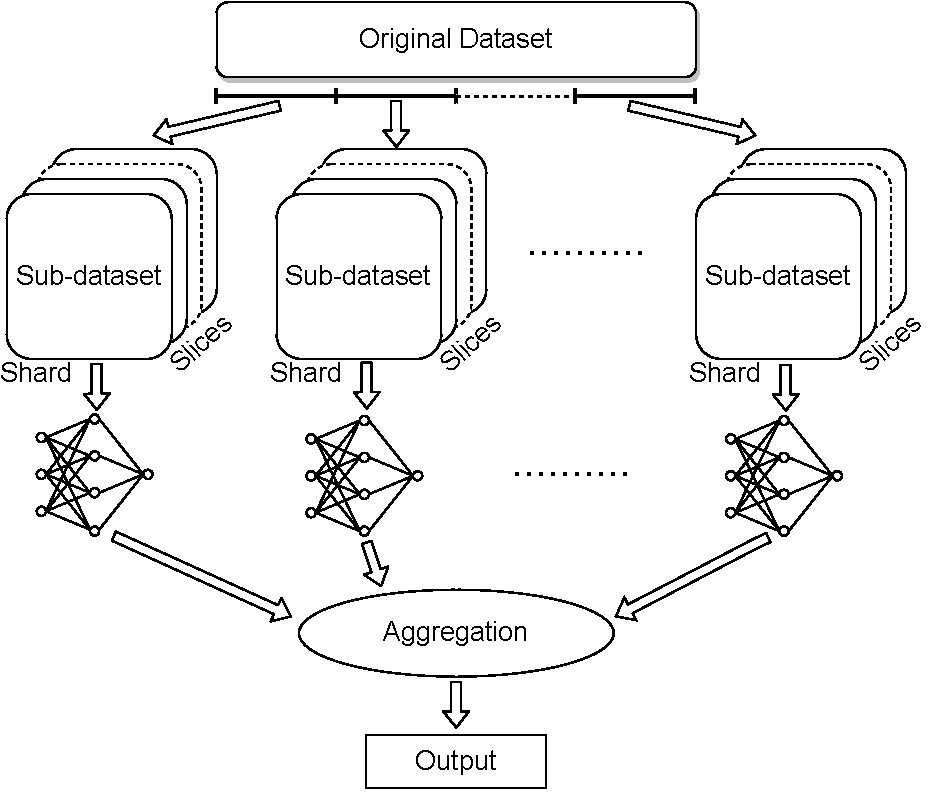
\includegraphics[width=1.0\linewidth]{assets/shidong_fig1.pdf}
  \caption{An overview framework of SISA. The dataset is first sharded into multiple shards. Each shard is further sliced into multiple slices. Each shard is put into a deep learning model trained by gradually increasing the number of slices. The output of the DL models is combined using a voting-based aggregation.}
  \label{fig:sisa}
\end{figure}


\subsubsection{SISA~\cite{sisa}} This is an exact machine unlearning method aiming to reduce the computational cost of the retraining process by employing a data partitioning technique. Figure~\ref{fig:sisa} briefly describes an overview framework of SISA. In the beginning, the original data $\mathcal{D}$ is split into $\mathcal{S}$ shards, such as $\cap_{i \in |\mathcal{S}|} D_i = \O$ and $\cup_{i \in |\mathcal{S}|} D_i = \mathcal{D}$.
Each shard $D_i \in \mathcal{D}$ is then further split into $K$ slices, i.e.,  $\cap_{k \in |K|} D_{ik} = \O$ and $\cup_{k \in |K|} D_{ik} = D_i$. 
A deep learning (DL) model is constructed on each shard. The DL model is updated by gradually increasing the number of slices. Note that all the parameters of the DL model are kept in storage. After finishing the training process, SISA contains multiple DL models. Finally, the output results are collected by employing a voting mechanism on a list of outputs of DL models. When RTBF requests arrive, SISA automatically locates the shards and the slices containing the deleted data $\mathcal{D}_u$. SISA then retrains the DL models of these shards from the particular cached stage, i.e., before the slices of the deleted data were put into the DL models.


\begin{figure}[htbp]
  \centering
  \begin{subfigure}[b]{0.235\textwidth}
         \centering
  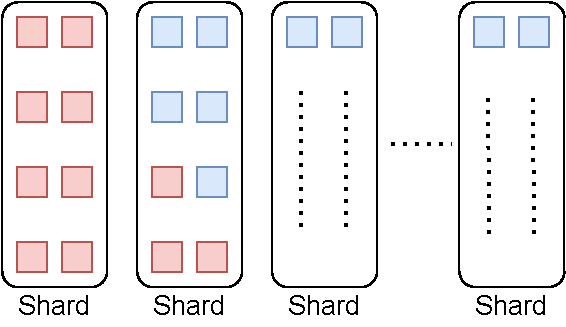
\includegraphics[width=0.95\linewidth]{assets/shidong-sisa-sharding.pdf}
  \caption{Instances with a higher deletion probability, illustrated as red squares, are allocated to the same shards so that when RTBF requests arrive, fewer shards are required to be retrained compared with the naive way of randomly allocating the instances.}
  \label{fig:sisa-sharding}
  \end{subfigure}
  \hspace{0.5mm}
  \begin{subfigure}[b]{0.235\textwidth}
  \centering
  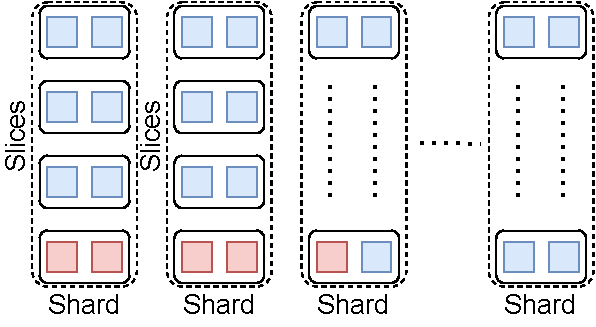
\includegraphics[width=\linewidth]{assets/shidong-sisa-slicing.pdf}
  \caption{Instances with high likelihood, illustrated as red squares, are placed in the last slices. When we receive the RTBF requests, the DL model of each shard is retrained from a checkpoint before those slices containing the deleted data are merged. 
  }
  
  \label{fig:sisa-slicing}
    \end{subfigure}
   \caption{SISA's strategies aim to reduce the computational cost of the retraining process.}
\end{figure}


The priori probability is the probability of an event happening when we have a limited number of possible outcomes that equally occur~\cite{leung2007naive}. Machine unlearning methods can easily improve their performance when we know the priori probability of data deletion from different groups. For example, wealthy families prefer to keep their privacy for safety purposes, so they tend to send RTBF requests compared to other people~\cite{upton2001strategic}. Another example is that people with a higher educational background are more likely to remove their personal information from public~\cite{eurobarometer}.

There are two strategies for SISA to leverage the priori probability to speed up the training process, hence reducing the computational cost. The first strategy is to allocate the instances with a higher deletion probability into the same shards. This means the retraining process would happen on fewer shards compared with randomly allocating the instances. The second strategy is to allocate the instances with a higher deletion probability to the last slices. In this case, the retraining process would happen on fewer slices compared with randomly allocating the instances. Figure~\ref{fig:sisa-sharding} and Figure~\ref{fig:sisa-slicing} briefly describe the first and second strategies, respectively.


SISA is efficient and effective in dealing with machine unlearning problems. The method has inspired many later works~\cite{recommendation, coded, graph-eraser}. Its source code is placed at \url{https://github.com/cleverhans-lab/machine-unlearning}.


\subsubsection{AmnesiacML~\cite{amnesiac}} This is a method of approximate machine unlearning approach. AmnesiacML makes use of the characteristics of batch training in neural networks. During the training process, the updated parameters of a DL model for each batch are recorded and kept in storage. The training process is expressed as follows:

\begin{equation}
\theta_{M} = \theta_{\mathrm{initial}} + \sum_{e=1}^{E}\sum_{b=1}^{B}\Delta_{\theta_{e,b}}
\label{amnesiac-formula}
\end{equation}
where $\theta_{\mathrm{initial}}$ is the initial parameters of the DL model, $E$ and $B$ represent the total number of epochs and the total number of batches in each epoch, respectively. The updated parameters are stored as $\{ \gamma_b \mid \gamma_b = \sum_{e=1}^E\Delta_{\theta_{e,b}} , 1 \leq b \leq B\}$.


When we receive the RTBF requests, AmnesiacML automatically locates the batches containing the instances that need to be deleted. After that, the DL model's parameters are rolled back to remove the impact of the deleted data on the trained DL model as follows: 

\begin{equation}
\theta_{M'} = \theta_{M} - \sum_{\hat{b}=1}^{\hat{B}}\gamma_{\hat{b}}
\label{amnesiac-update}
\end{equation}

A strategy for AmnesiacML is easily adopted when we comprehend the priori probability of deleted data from different groups. For example, instances with a higher priori probability of being removed can be placed into the same batches. Hence, the process of updating parameters in the DL model will require a less computational cost. 


Similar to SISA, AmnesiacML shows its efficiency and effectiveness in machine unlearning problems. However, it does not ensure the impact of deleted data being completely forgotten in the updated DL model. The open-source repository of AmnesiacML can be found at \url{https://github.com/lmgraves/AmnesiacML}


\subsection{AI Fairness Metrics}
\label{sec:ai_metrics}


The goal of AI fairness is to correct machine learning (ML) models with the assumption that models should not be biased between any protected classes, i.e., race, sex, familial status, etc. Each protected class partitions a population into different groups, such as the privileged group and the unprivileged group. 
In this section, we employ four different fairness metrics, such as disparate impact, statistical parity difference, average odds difference, and equal opportunity difference, to evaluate the impact of machine unlearning methods on fairness. These metrics are widely adopted in measuring the fairness of ML systems~\cite{fairness-re, RE-AI, fairness-survey, fairness-testing, zhang2021ignorance, biswas2020machine, dwork2012fairness, chakraborty2020fairway}.

Let $x_s \in \{0, 1\}$ indicates the binary label of a protected class ($x_s = 1$ for the privileged group). Let $\hat{y} \in \{0, 1\}$ be the predicted outcome of a ML classification model ($\hat{y}=1$ for the favourable decision). Let $y \in \{0, 1\}$ be the binary classification label ($y=1$ is favourable). We present the four fairness evaluation metrics as follows. 


\noindent \textbf{Disparate impact (DI)}~\cite{di} measures the ratio of the favourable outcome of the unprivileged group ($x_s=0$) against the privileged group ($x_s=1$). 
\begin{equation}
    \frac{P[\hat{y} = 1 \mid x_s = 0]}{P[\hat{y} = 1 \mid x_s = 1]}
\label{di-formula}
\end{equation}



\noindent \textbf{Statistical parity difference (SPD)}~\cite{spd} is the difference of the favourable outcome of the unprivileged group ($x_s=0$) against the privileged group ($x_s=1$). 
\begin{equation}
    P[\hat{y} = 1 \mid x_s = 0] - P[\hat{y} = 1 \mid x_s = 1]
\label{spd-formula}
\end{equation}

\noindent\textbf{Average odds difference (AOD)}~\cite{equal-op} calculates the average of difference in true positive rate and false positive rate between unprivileged and privileged groups. 
\begin{equation}
\begin{split}
    \frac{1}{2} (\lvert P[\hat{y} = 1|x_s = 0, y=1] - P[\hat{y} = 1|x_s = 1, y=1] \rvert \\
    +\lvert P[\hat{y} = 1|x_s = 0, y=0] - P[\hat{y} = 1|x_s = 1, y=0]\rvert)
\end{split}
\label{aod-formula}
\end{equation}


\noindent \textbf{Equal opportunity difference (EOD)}~\cite{equal-op} evaluates the difference in true positive rate between unprivileged group and privileged groups.
\begin{equation}
    P[\hat{y} = 1|x_s = 0, y=1] - P[\hat{y} = 1|x_s = 1, y=1]
\label{eod-formula}
\end{equation}

All fairness metrics are range from -1 to 1. Among them, DI achieves the greatest fairness of the classification model when it equals 1. The remaining fairness metrics, i.e., SPD, AOD, and EOD, attain the greatest fairness when their values are 0.



